% ? mins environs

% ------------------------- %

\begin{frame}
\frametitle{Contexte de travail (1/4)}
\framesubtitle{Caract�ristiques g�n�rales de la carte acoustique}
	\begin{figure}
	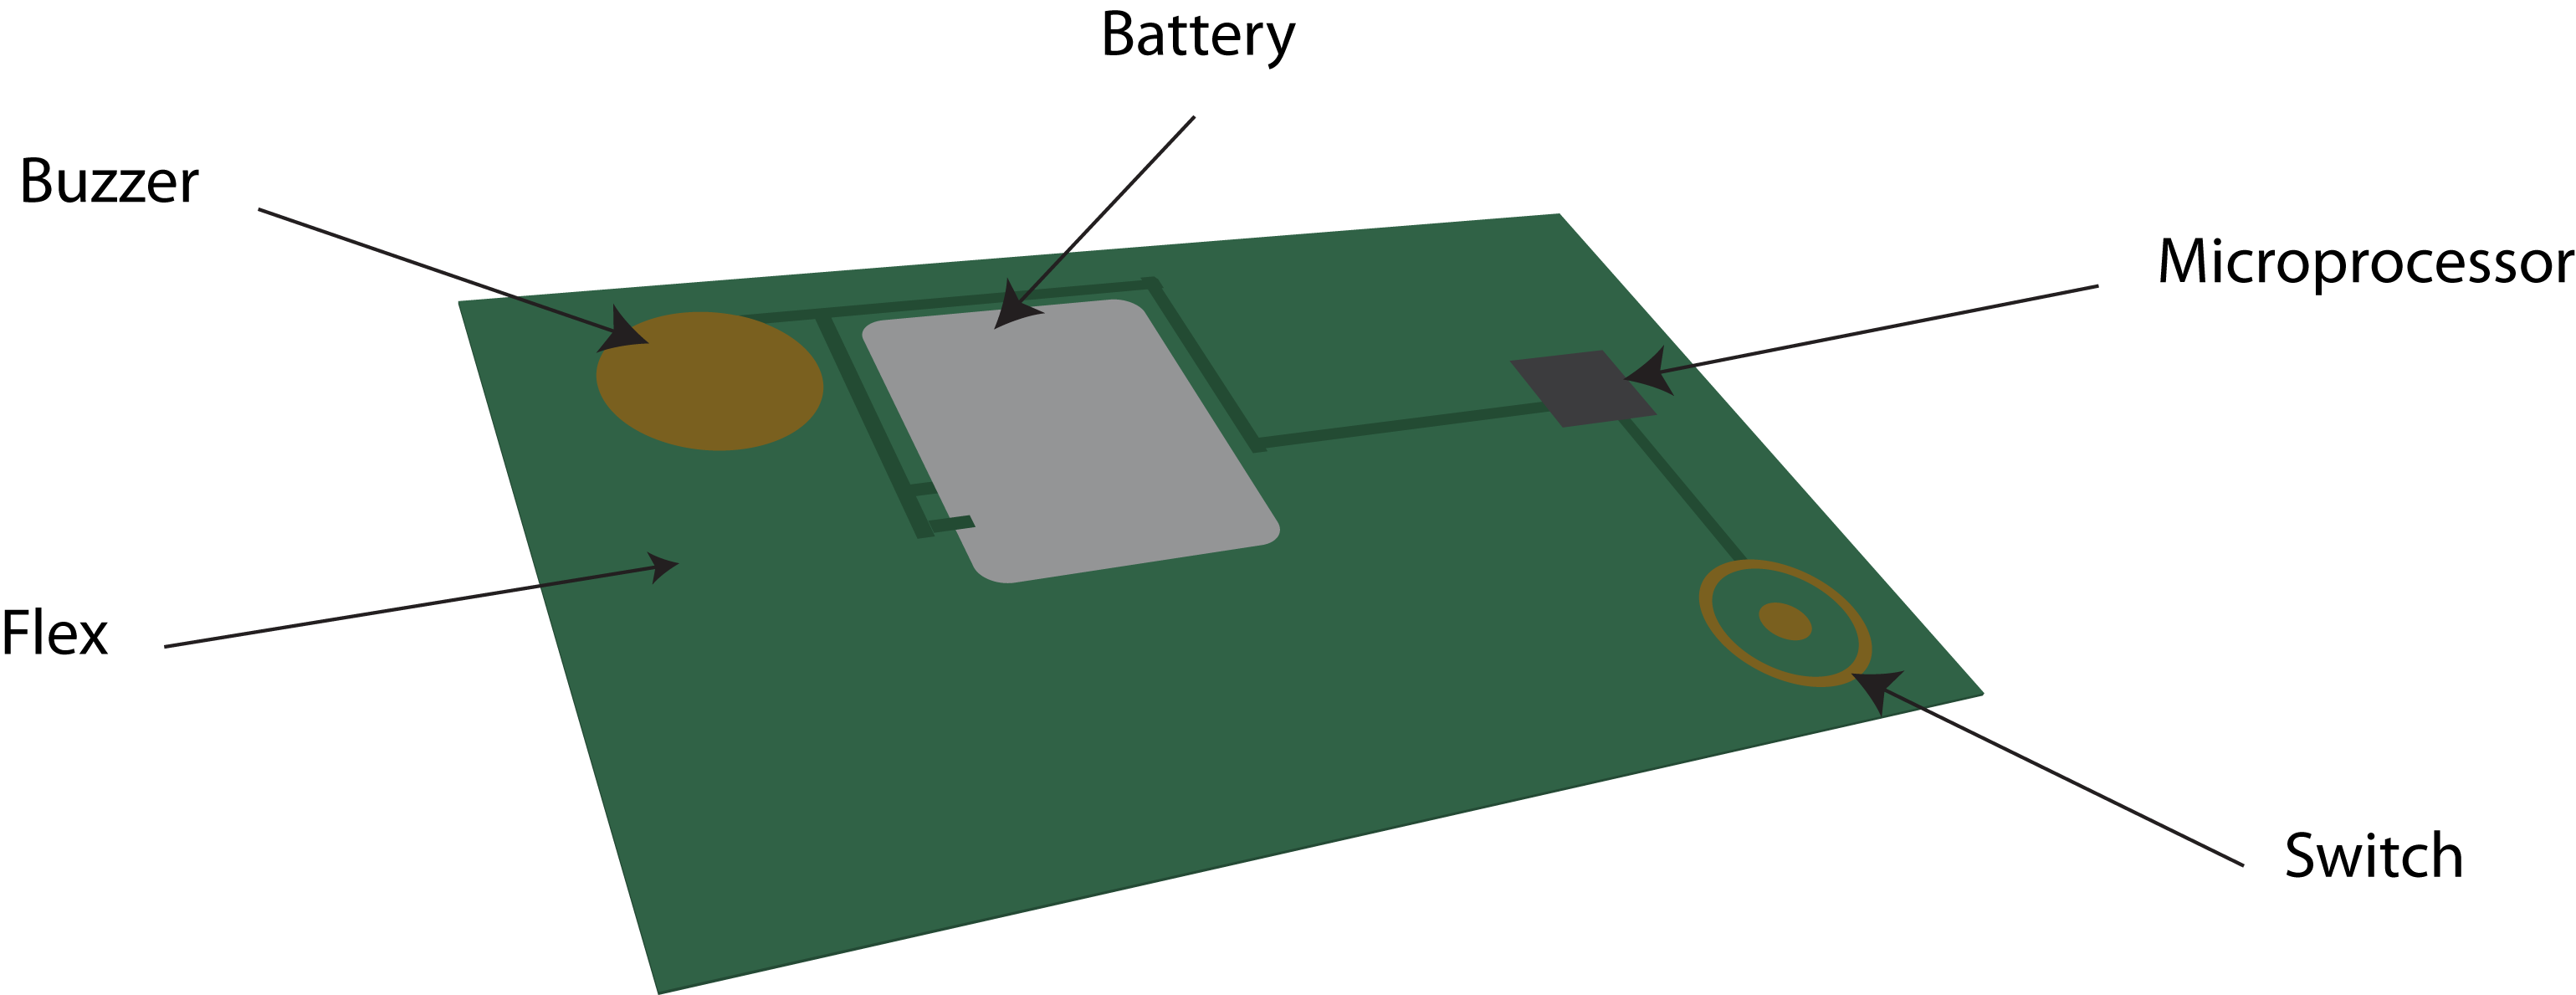
\includegraphics[scale = 0.3]{images/carteinside}	
	%\caption{Sch�ma d'une carte acoustique}
	\end{figure}

	\begin{block}{L'�lectronique embarqu�e est compos�e des �l�ments}
	\begin{itemize}
	\item Int�gr�s sur un circuit imprim� flexible, ou � flex �
	\item Soud�s au � flex � par un processus de capillarit�
	\item Flex composants est appel� Inlay
	\item Int�gr� � l'int�rieur de la carte PVC
	\end{itemize}
	\end{block}
\end{frame}

% ------------------------- %
\begin{frame}
\frametitle{Contexte de travail (2/4)}
\framesubtitle{Caract�ristiques g�n�rales de la carte acoustique}
\centering
Organigramme de fonctionnement de la carte acoustique
	\begin{figure}
	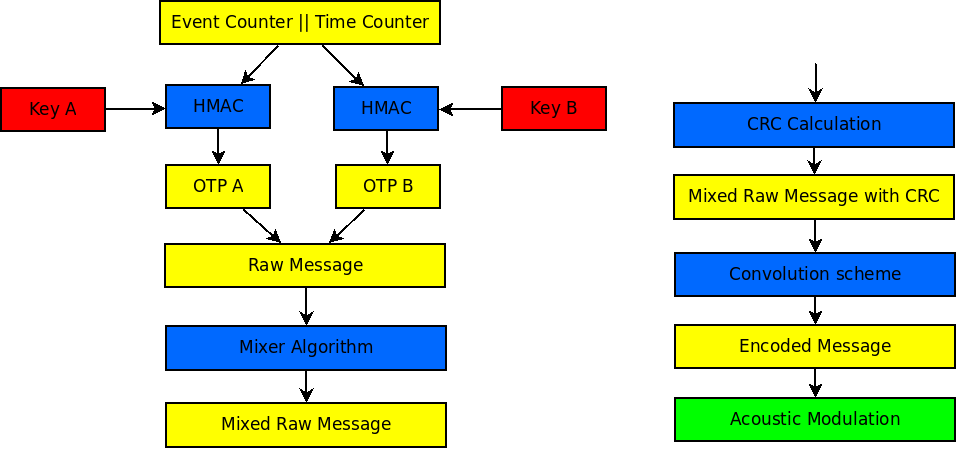
\includegraphics[scale = 0.3]{images/organigramme2}	
	\caption{Fonctionnement de la carte acoustique}
	\end{figure}
\end{frame}

% ------------------------- %
\begin{frame}%[plain]
\frametitle{Contexte de travail (3/4)}
\framesubtitle{Caract�ristiques g�n�rales de la carte acoustique}
	\begin{block}{Les constantes et variables essentielles}
	\begin{itemize}
	\item Les cl�s cryptographiques (HOTP KeyA \& HOTP KeyB) 
	\item Le compteur d'�v�nements (Event Counter) 
	\item Le num�ro de s�rie (Id)
	\end{itemize}
	\end{block}

	\begin{exampleblock}{G�n�ration du cryptogramme acoustique}
	\begin{itemize}
	\item La g�n�ration d'un HOTP et du cryptogramme
	\item L'encodage du cryptogramme 
	\begin{itemize}
		\item Le cryptogramme et les symboles
		\item Le m�langeur
		\item L'ajout du CRC16 au message 
		\item Le codage convolutif 
	\end{itemize}
	\item La restitution du cryptogramme 
	\end{itemize}
	\end{exampleblock}

\end{frame}


% ------------------------- %
\begin{frame}
\frametitle{Contexte de travail (4/4)}
\framesubtitle{Caract�ristiques g�n�rales de la carte acoustique}
	\begin{block}{Les trois versions}
	\begin{itemize}
	\item \textbf{V4G}
	\item V0 
	\item V1
	\end{itemize}
	\end{block}

	\begin{exampleblock}{Les outils}
	\begin{itemize}
	\item Offline: L'utilitaire \textit{ListenAcousticMessage\_V1.2.1.35.exe}
	\item Online: \href{http://solution.uint.info/Acoustictechno/}{La page de test}
	\item Authentification (SAS)
	\end{itemize}
	\end{exampleblock}
\end{frame}


